\chapter{Численные эксперименты}
\section{Параметры БЛА}
Для подтверждения работоспособности синтезированной системы управления создана модель в прикладном пакете Matlab Simulink и проведены вычислительные эксперименты. Параметры модели приведены в Таблице \ref{tb:params_table}.
\begin{table}[h!]
	\centering
	\caption{ -- Параметры модели}\label{tb:params_table} 
	\begin{tabular}{lcl}
		\hline
		Параметр & Обозначение & Значение  \\\hline
		Общая масса & $M$ & 2,0 кг  \\
		Тензор инерции корпуса & $\bm J_B$ & $diag(2e^{-2}, 2e^{-2}, 4e^{-2})$ кг$\cdot$м$^2$  \\
		Тензор инерции ротора & $\bm J_R$ & $diag(2e^{-5}, 2e^{-5}, 1e^{-5})$ кг$\cdot$м$^2$  \\
		Миделево сечение корпуса & $S_{\perp}$ & 0,12 м$^2$ \\
		Луч & $L$ & 0,25 м \\
		Аэродинамический коэффициент & $C$ & 1,05\\
		Аэродинамический коэффициент & $k$ & 1,13$\cdot 10^{-5}$ Н$\cdot$с$^2\cdot$рад$^{-2}$ \\		
		Аэродинамический коэффициент & $b$ & 1,5$\cdot 10^{-6}$ Н$\cdot$м$\cdot$с$^2\cdot$рад$^{-2}$ \\		
		Максимальные обороты & $\tilde \omega_{max}$ & 1140 рад/с \\		
		Максимальный угол & $\theta_{max}$ & ${\pi}/{3}$ рад \\
		Константа балансировки & $\epsilon_\tau$ &6 Н$\cdot$м \\
		\hline
	\end{tabular}
\end{table}

На основе приведенных выше параметров динамики были рассчитаны параметры ограничений с использованим алгоритма, описанного в разделе \ref{section:limits}. Сначала было выбрано направление диагонали прямоугольной области $\Psi_{\boldsymbol{y}}$ таким образом, чтобы ограниченные таким способом выходы регулятора \eqref{eq:m_reg} в достаточной степени удовлетворяли разумному соотношению маневренных качеств БЛА. Как было отмечено ранее, выбор данного направления обусловлен конкретными задачами, которые предстоит решать с помощью мультироторного робота и является настроечным параметром системы управления. Для конфигурации, представленной параметрами, изложенными в Таблице \ref{tb:params_table}, можно выбрать
$$\bm d = (0,577, 0,577, 0,577, 0,014, 0,014, 0,014).$$
Для выбранной диагонали можно рассчитать значения пределов ограничений \eqref{eq:lims_final} и балансировочных параметров, входящих в дополняющие модель \eqref{eq:m_dyn} уравнения \ref{eq:m_dyn_balance_1}, \ref{eq:m_dyn_balance_2}. Результаты приведены в Таблице \ref{tb:lims_table}.
\begin{table}[h!]
	\centering
	\caption{Параметры ограничений}\label{tb:lims_table} 
	\begin{tabular}{lcl}
		\hline	
		Длина диагонали & $2\gamma^*$ & $28$ \\
		Константа балансировки & $\epsilon_T$ &2,6 Н$\cdot$м \\
		Константа балансировки & $\epsilon_F$ &0 Н\\
		\hline
	\end{tabular}
\end{table}
Таким образом выполнение имеющихся ограничений параметров системы исполнительных органов управления на максимальные обороты двигателей
$\tilde \omega_{max}$ = 1140 рад/с
и на максимальные углы отклонения роторов с пропелерами от вертикали
$\theta_{max}$ = ${\pi}/{3}$ рад,
ограничивает максимально возможнок целевое ускорение БЛА по каждой из осей значением
$\ddot {\bm r}_{max}^0 \approx 4$ м/с$^2$,
угловое ускорение вдоль осей $X$ и $Y$ значением
$\dot {\bm \Omega}_{max}^0 \approx 10$ рад/с$^2$
и угловое ускорение вдоль оси $Z$ значением
$\dot {\tilde{\bm \Omega}}_{max}^0 \approx 5$ рад/с$^2$.

\section{Выполнение летного задания}
В эксперименте аппарат должен выполнить наблюдение за подвижным объектом, летя неподалеку от него и ориентируя камеру, установленную спереди, так, чтобы объект находился в центре полученного изображения.
Мы не рассматриваем вопрос построения траектории БЛА, считая ее определённой заранее.
Точка старта аппарата расположена на расстоянии 90 метров от цели, затем оно постепенно сокращается до 50 метров.
Траектория БЛА и наблюдаемого объекта изображены на рисунке \ref{fig:mau_traj}.
\begin{figure}[h!]
	\centering
	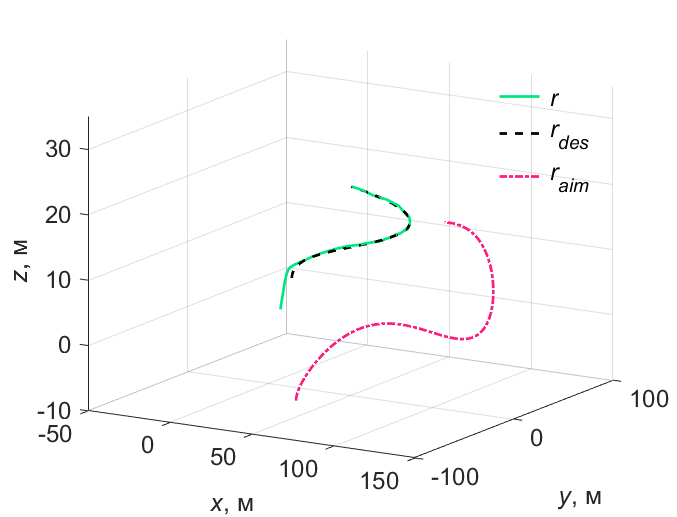
\includegraphics[width=16cm]{traj.png}
	\caption{ -- Траектории: целевая БЛА (черная пунктирная линия), БЛА (зеленая линия), наблюдаемого объекта (красная линия)}
	\label{fig:mau_traj}
\end{figure}

\begin{comment}
На рисунках \ref{fig:mau_eul} представлены углы ориентации квадрокоптера во время движения.
\begin{figure}[h!]

\subfloat[Крен]{%
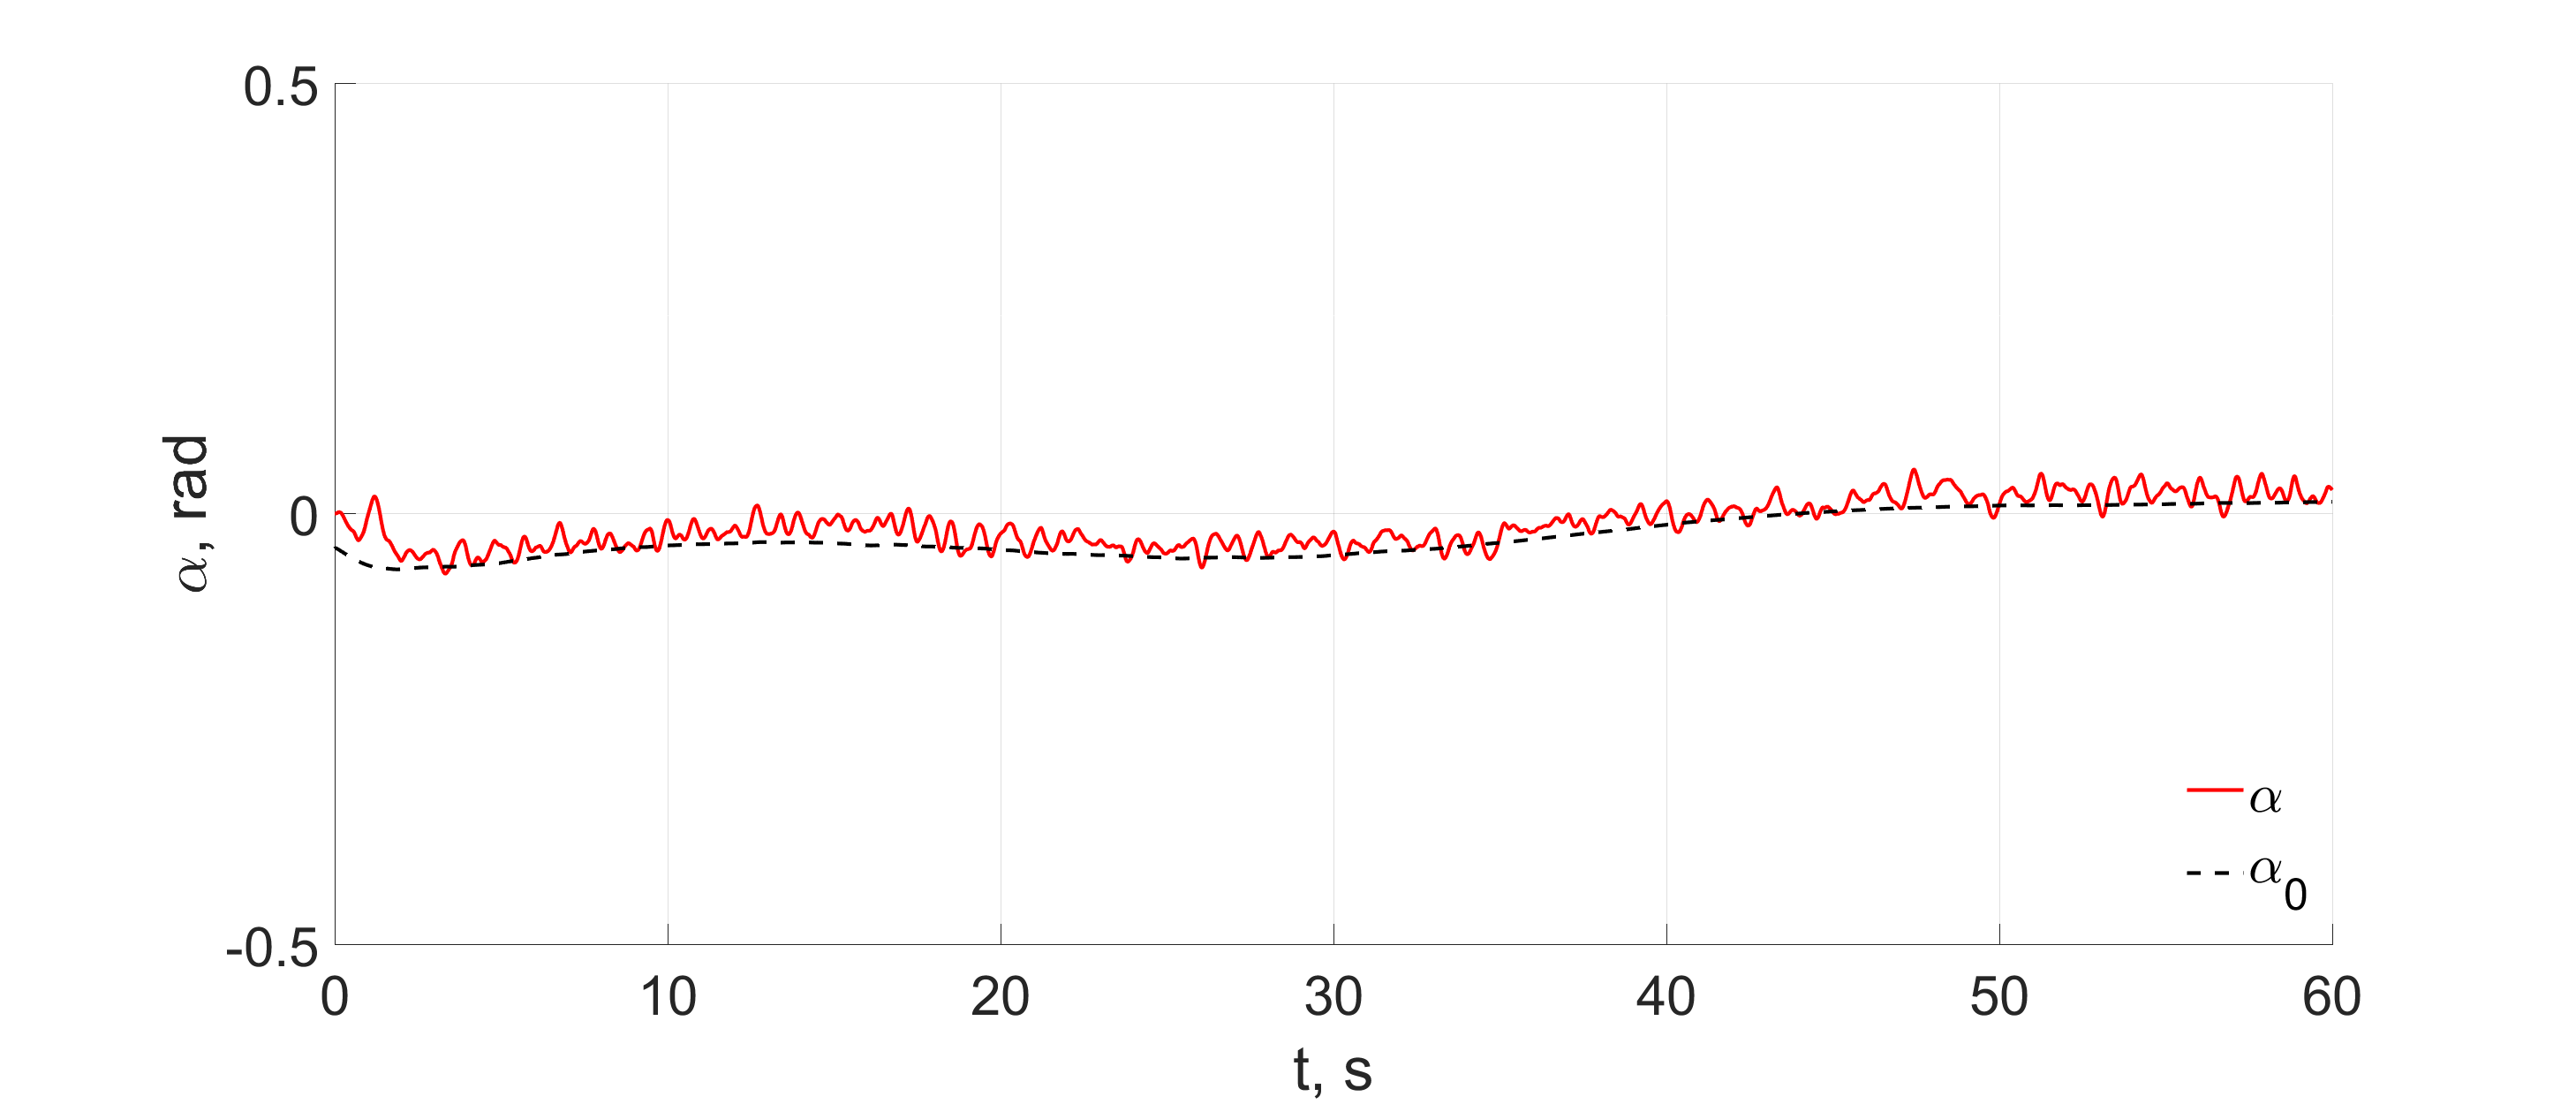
\includegraphics[clip,width=0.9\columnwidth]{roll}%
}

\subfloat[Тангаж]{%
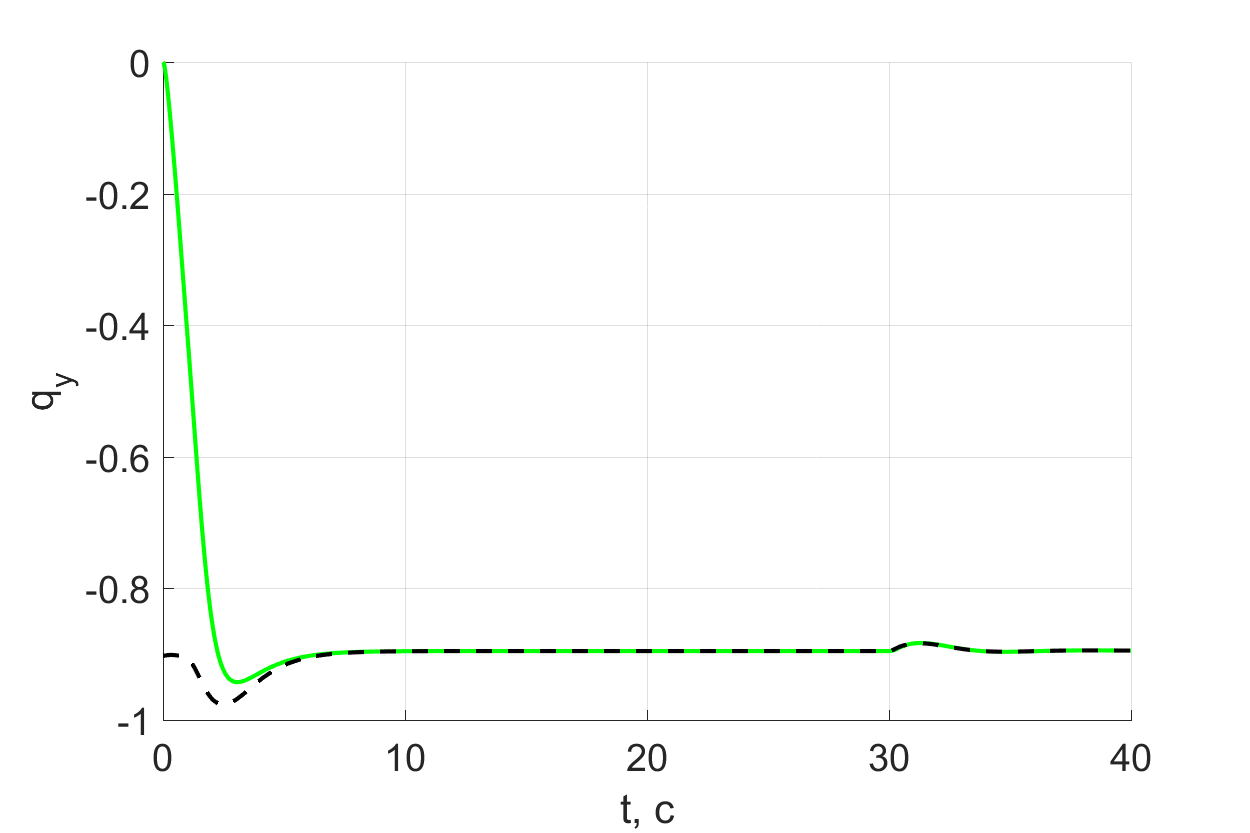
\includegraphics[clip,width=0.9\columnwidth]{pitch}%
}

\subfloat[Рысканье]{%
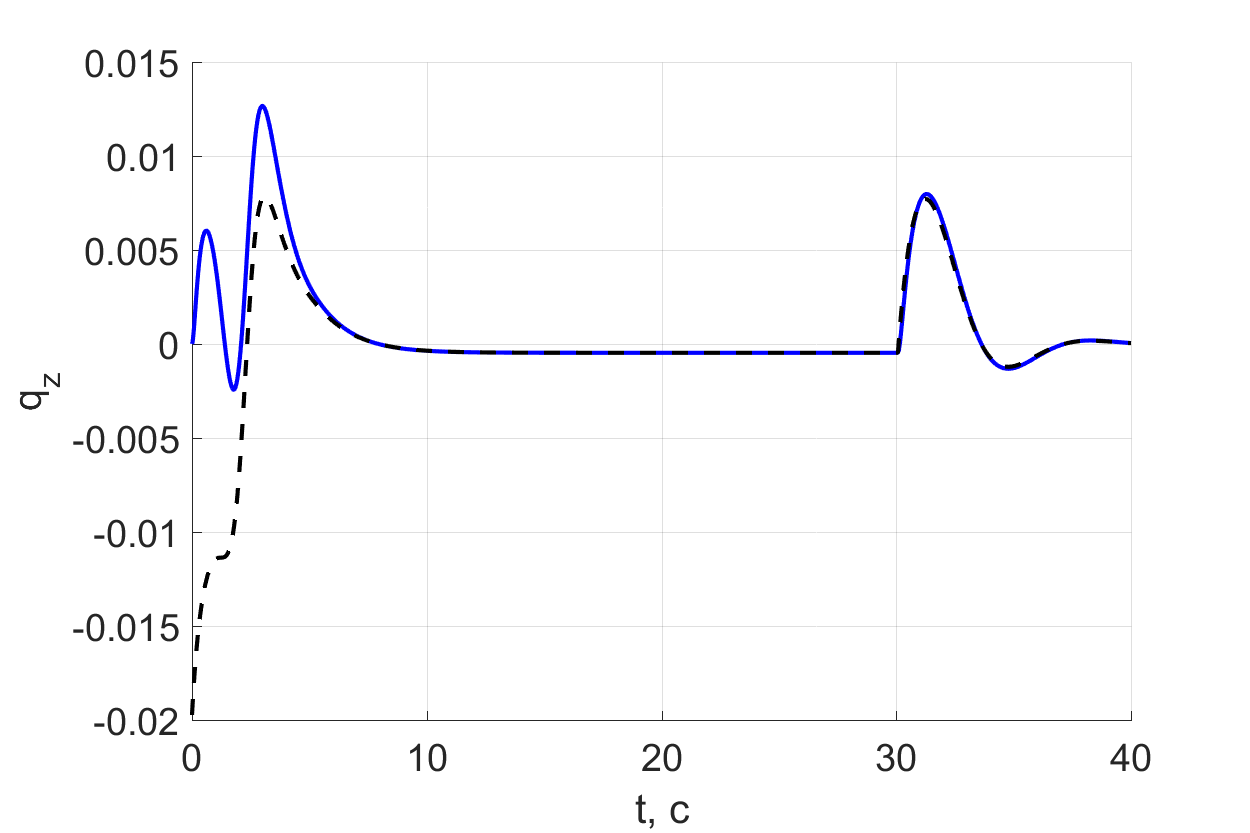
\includegraphics[clip,width=0.9\columnwidth]{yaw}%
}
\caption{ -- Углы ориентации}
\label{fig:mau_eul}

\end{figure} 
\end{comment}

На рисунке \ref{fig:mau_errors}, на графиках слева, изображены ошибки ориентации по углам крена, тангажа и рысканья (красная, зеленая и синяя линии соответственно), а также справа -- ошибки положения  квадрокоптера по осям $X$, $Y$ и $Z$ (красная, зеленая и синяя линии соответственно).
Ошибки по каждому из углов ориентации после стабилизации не превышают пяти градусов.
После выхода аппарата на целевую кривую максимальное абсолютное отклонение от траектории составило чуть более полуметра, что видно из графика абсолютной ошибки от времени (см. рис. \ref{fig:mau_abs_dr}).
\begin{figure}[h!]
	\centering
	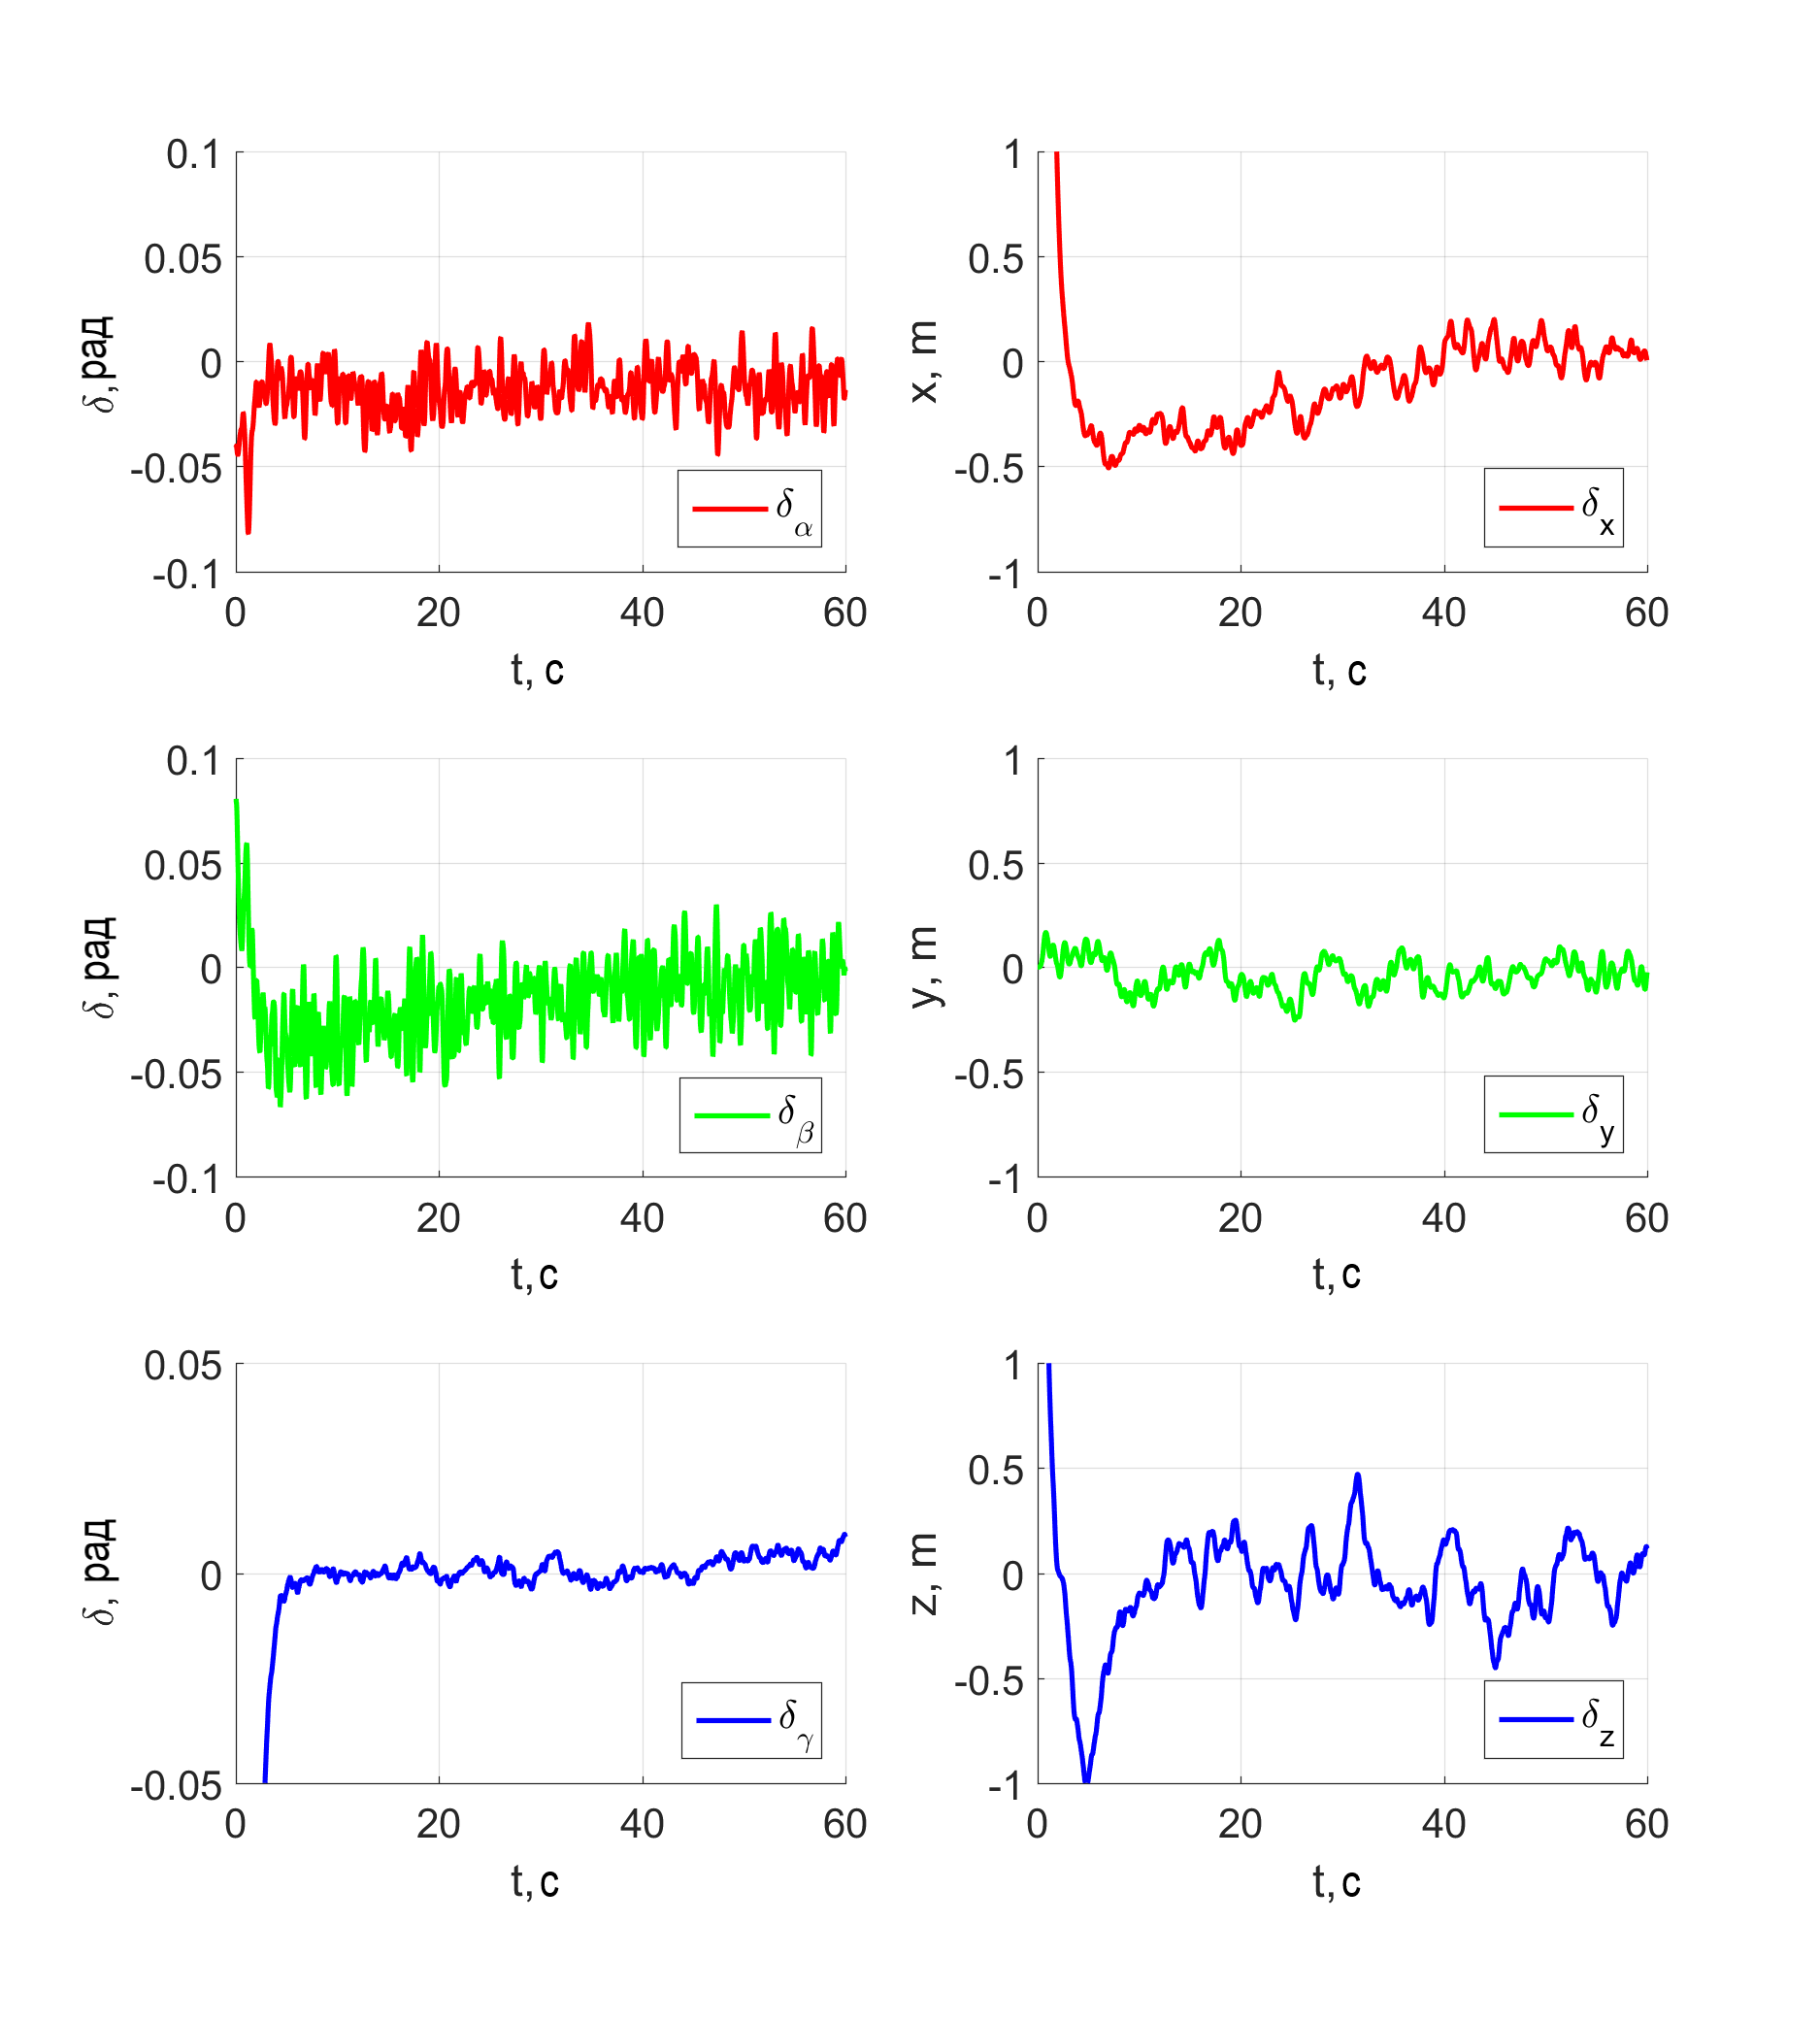
\includegraphics[width=16cm]{errors_rows.png}
	\caption{ -- Ошибка ориентации и позиции}
	\label{fig:mau_errors}
\end{figure}

\begin{figure}[h!]
	\centering
	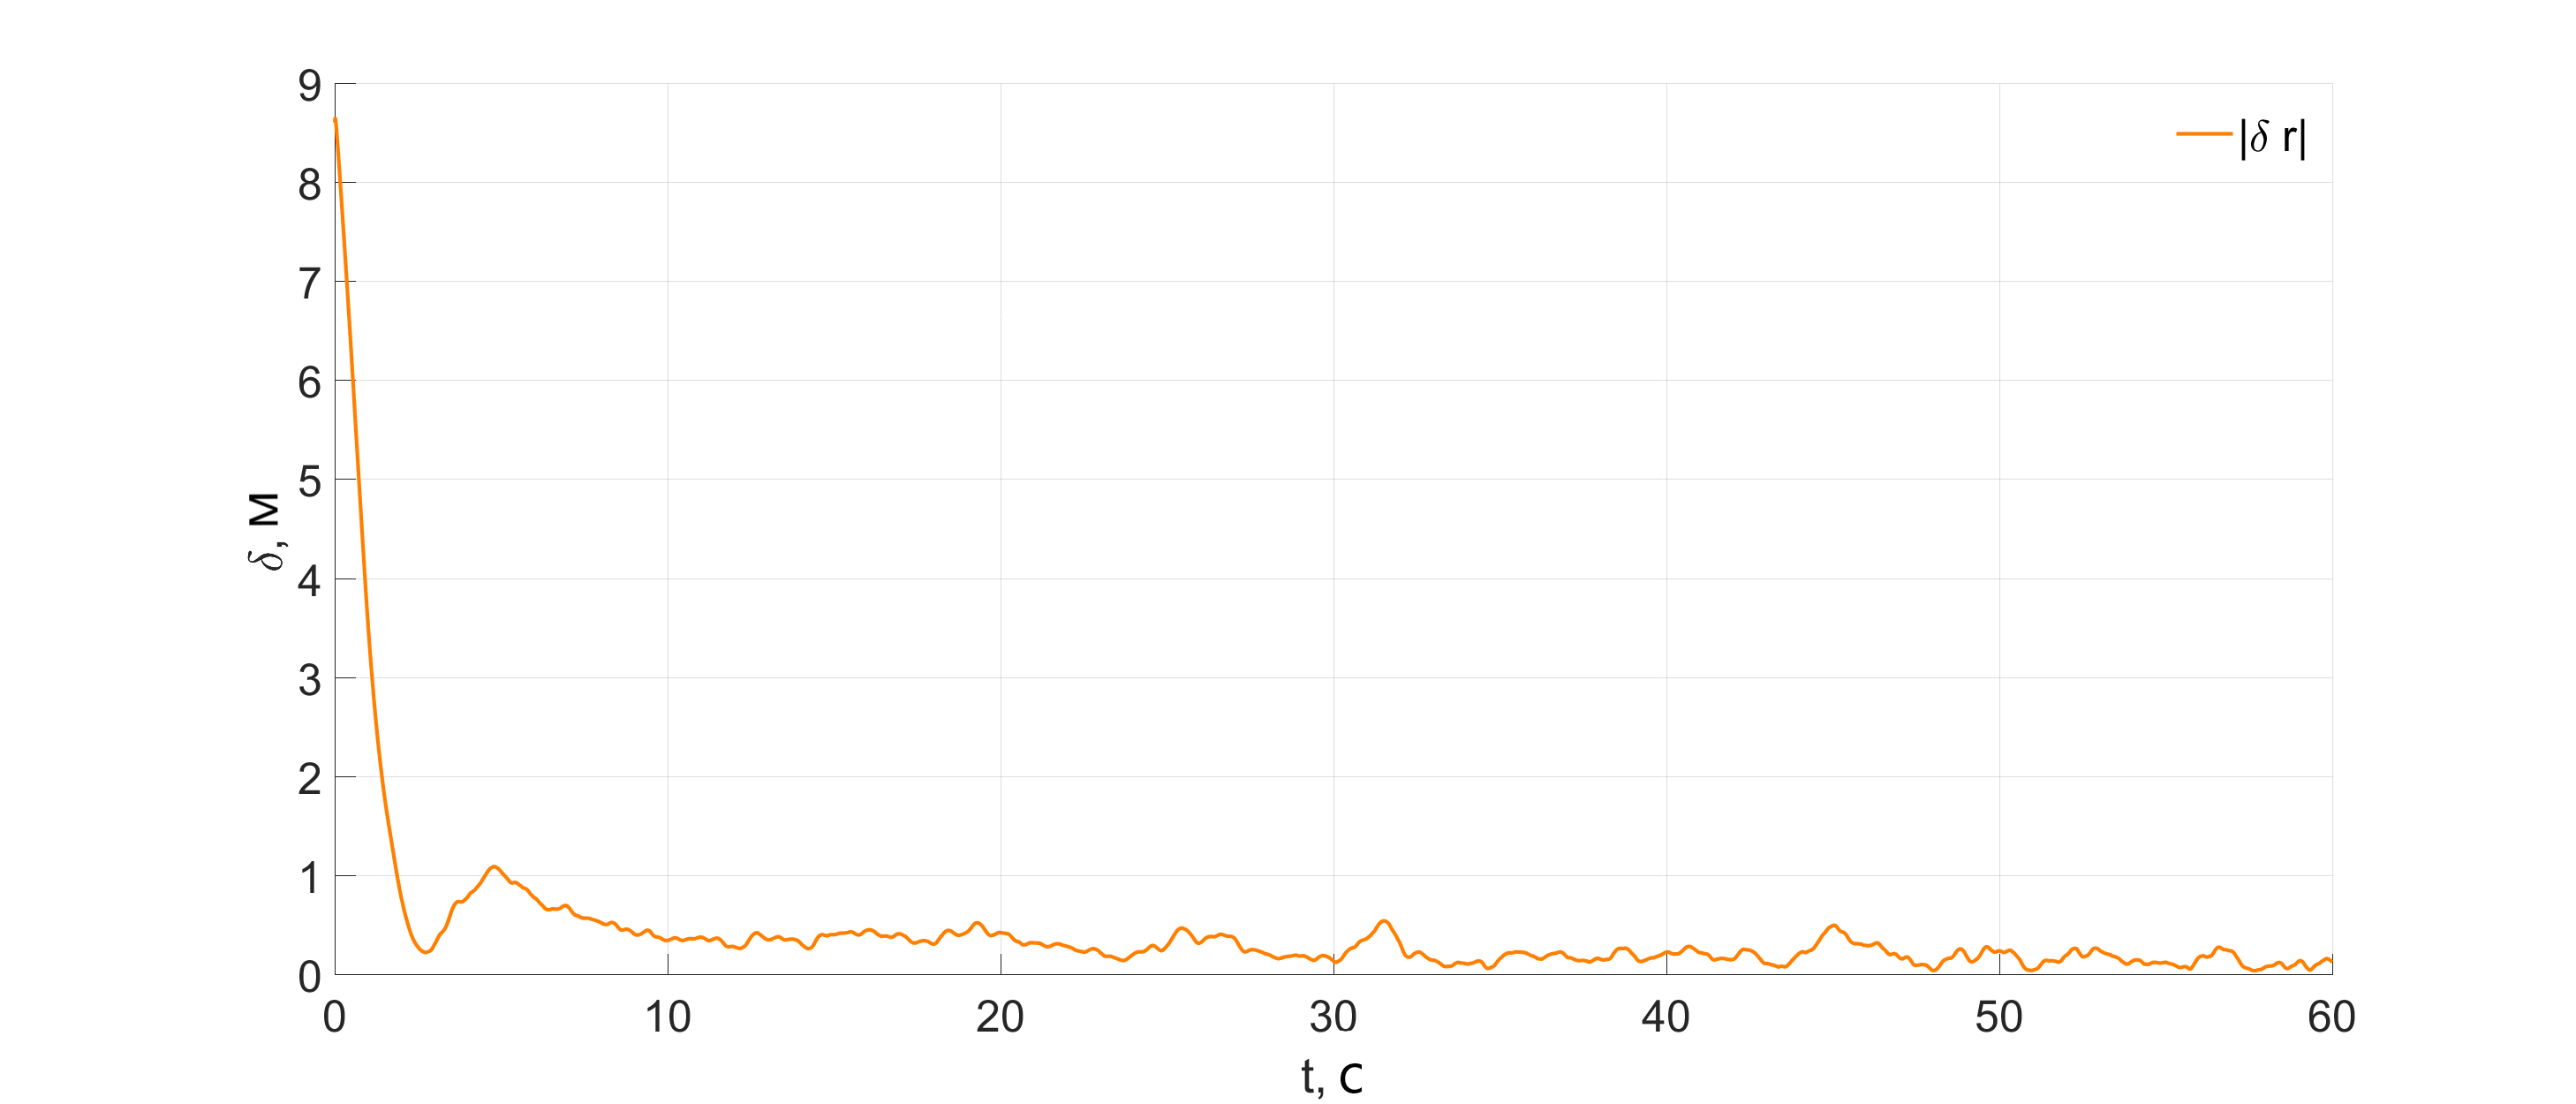
\includegraphics[width=16cm]{abs_dr}
	\caption{ -- Абсолютная ошибка позиции}
	\label{fig:mau_abs_dr}
\end{figure}

На рисунке \ref{fig:mau_cam} можно проследить за траекторией наблюдаемого объекта на записи, которою можно сделать с помощью передней камеры.
Видно, что в начальный момент времени объект находится вне зоны видимости, затем перемещается в центр экрана и далее на протяжении всего времени манёвра ось визирования камеры отклоняется от направления на объект не более чем на 4 градуса.
\begin{figure}[h!]
	\centering
	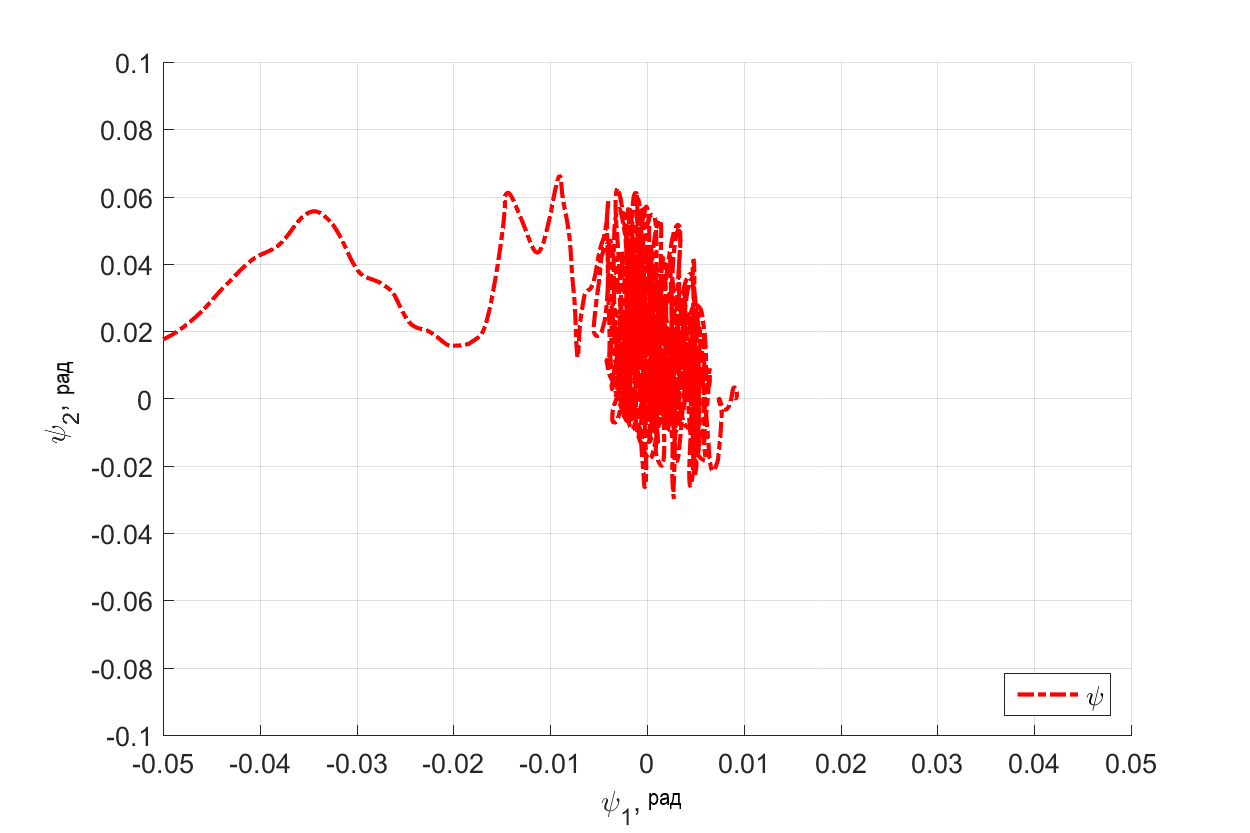
\includegraphics[width=16cm]{camera.png}
	\caption{ -- Траектория объекта на записи}
	\label{fig:mau_cam}
\end{figure}

Рисунок \ref{fig:mau_est} демонстрирует производительность алгоритмов оценки состояния. Слева приведены графики ошибки оценки углов крена, тангажа и рысканья (красная, зеленая и синяя линии соответственно) и их прямых измерений (серые линии). Справа – оценка положения по осям $X$, $Y$ и $Z$ (красная, зеленая и синяя линии соответственно) и их прямые измерения (серые линии).
\begin{figure}[h!]
	\centering
	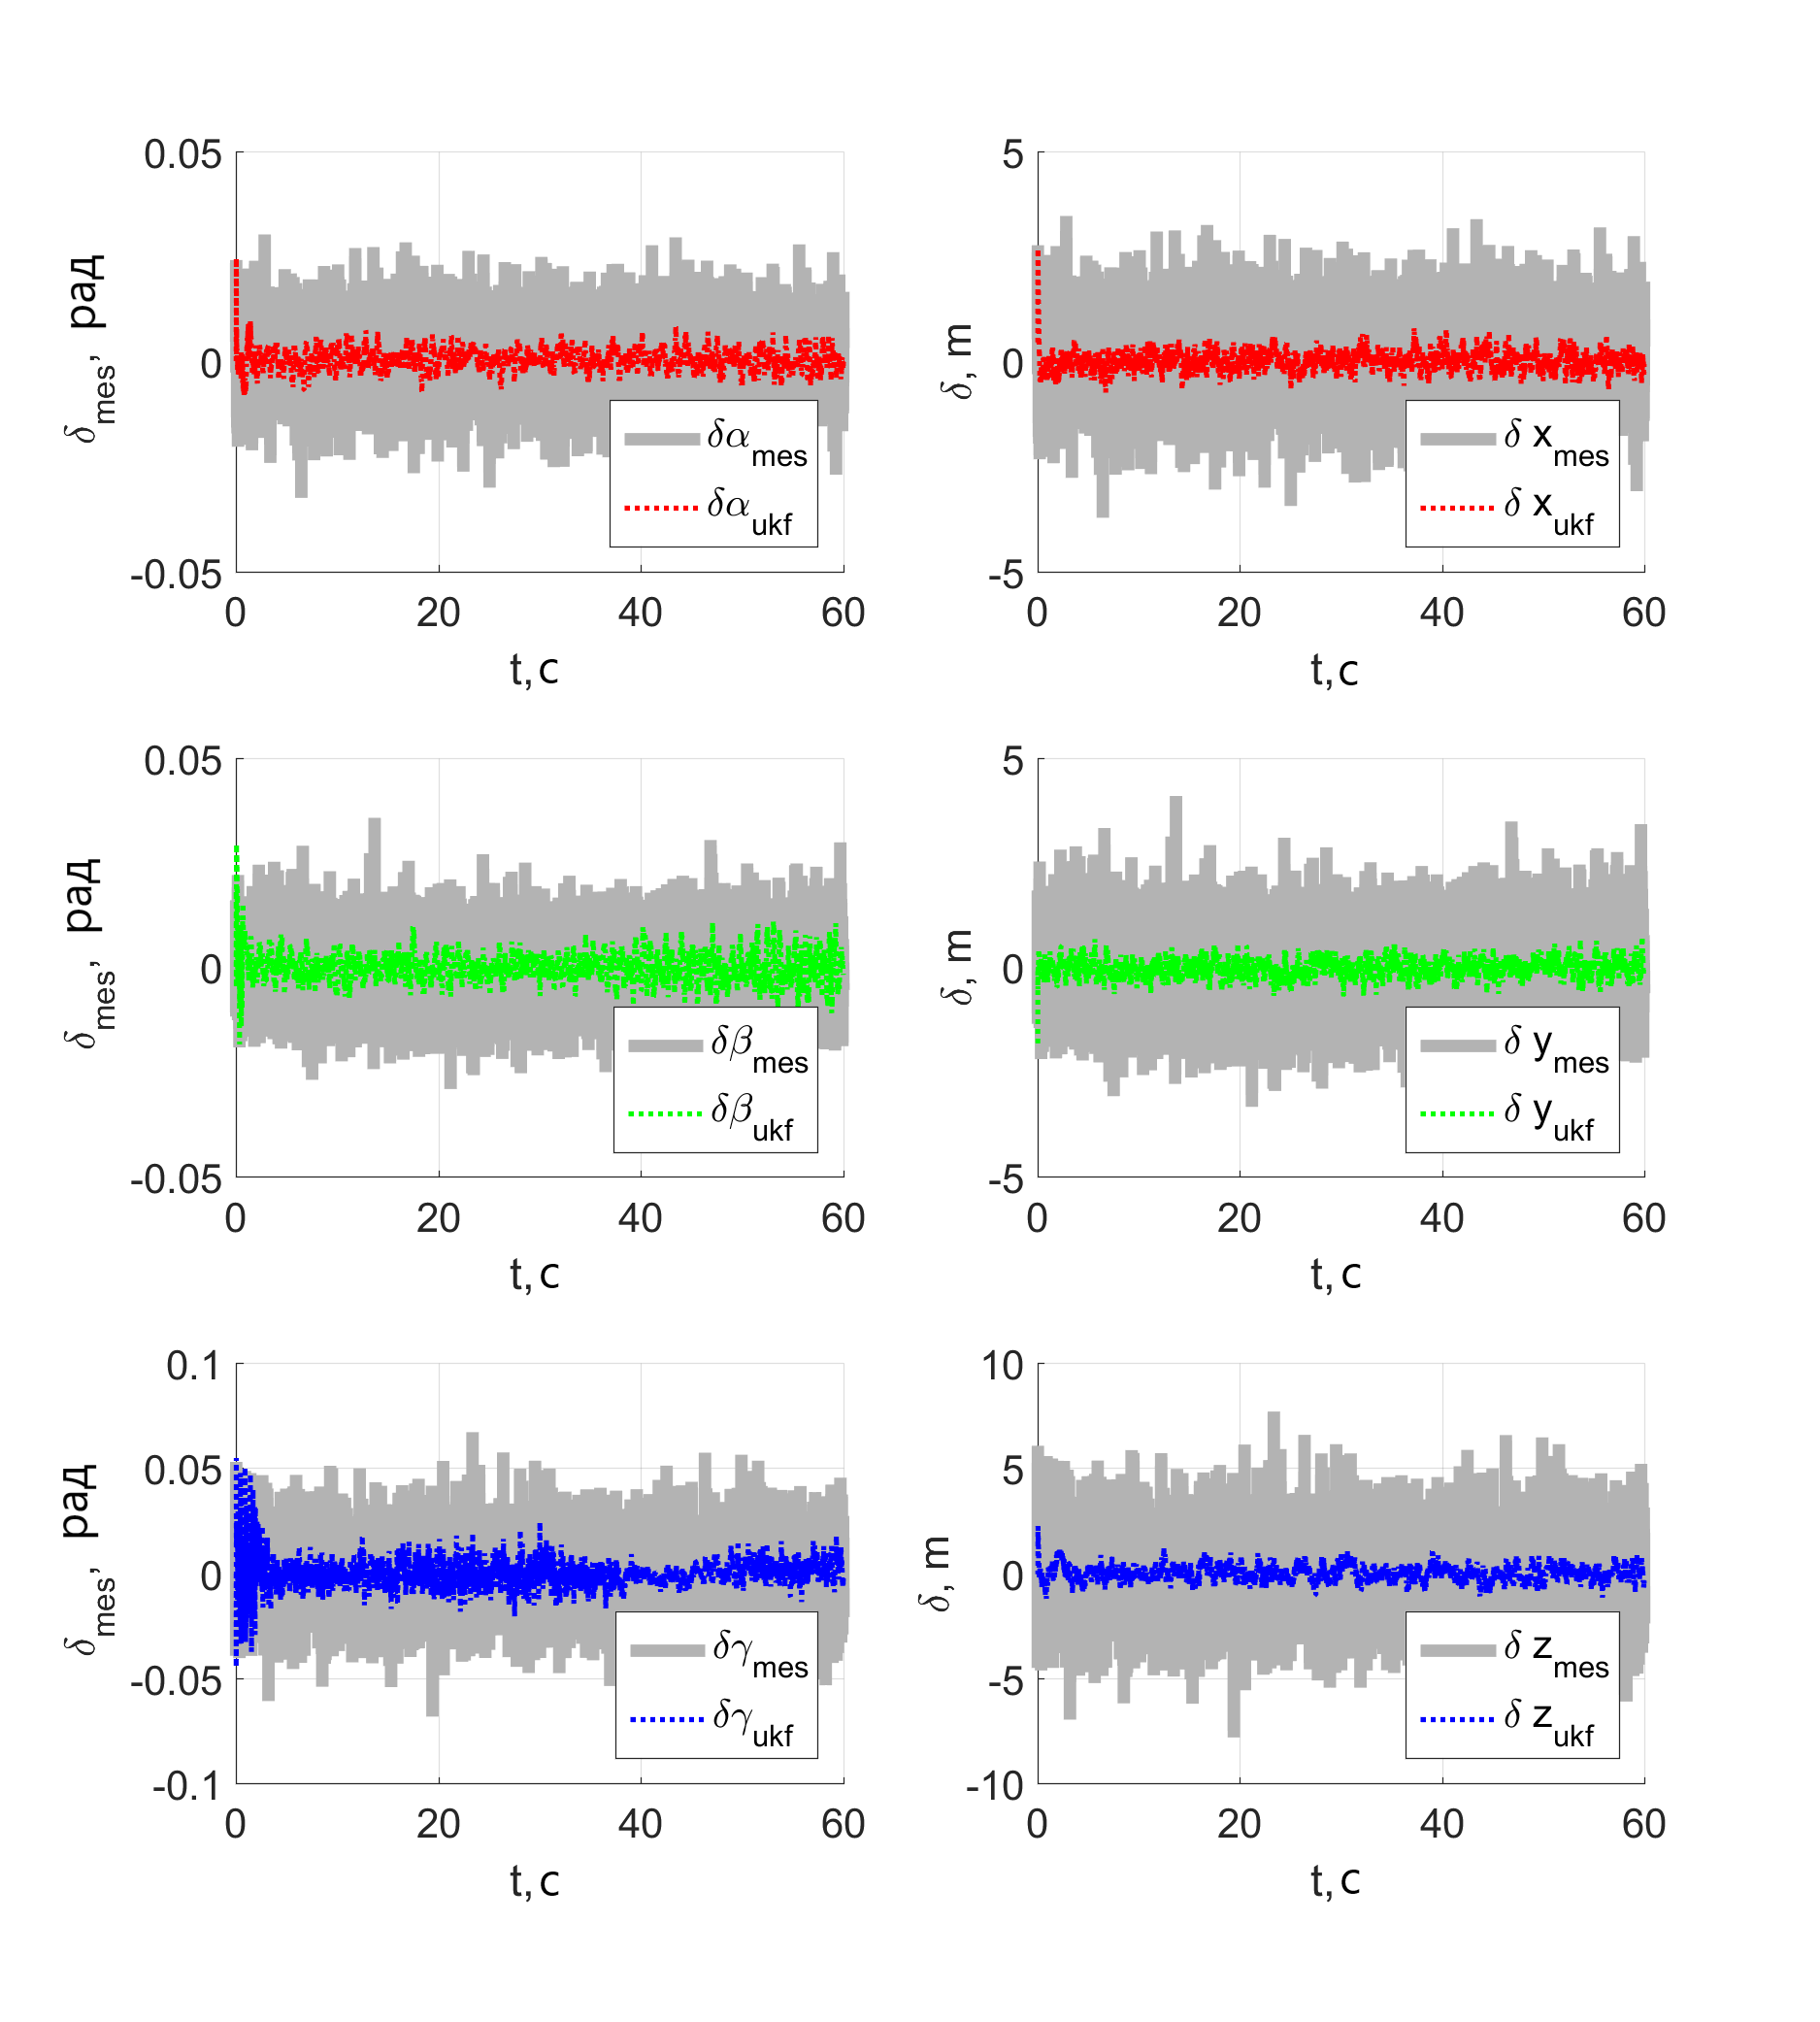
\includegraphics[width=16cm]{est_meas.png}
	\caption{ -- Ошибка оценки состояния и прямых измерений}
	\label{fig:mau_est}
\end{figure}
Алгоритмы фильтрации позволяют значительно снизить уровень шума измерений текущей позиции. Среднеквадратичная ошибка оценки ориента-ции составила менее одного градуса.

На графиках, изображенных на рисунке \ref{fig:mau_ctrl_out} представлены компоненты вектора управляющих параметров, которые, как легко заметить, лежат внутри выбранной ограниченной области

\begin{figure}[h!]
	
	\subfloat[Скорость вращения двигателей с пропеллерами]{%
		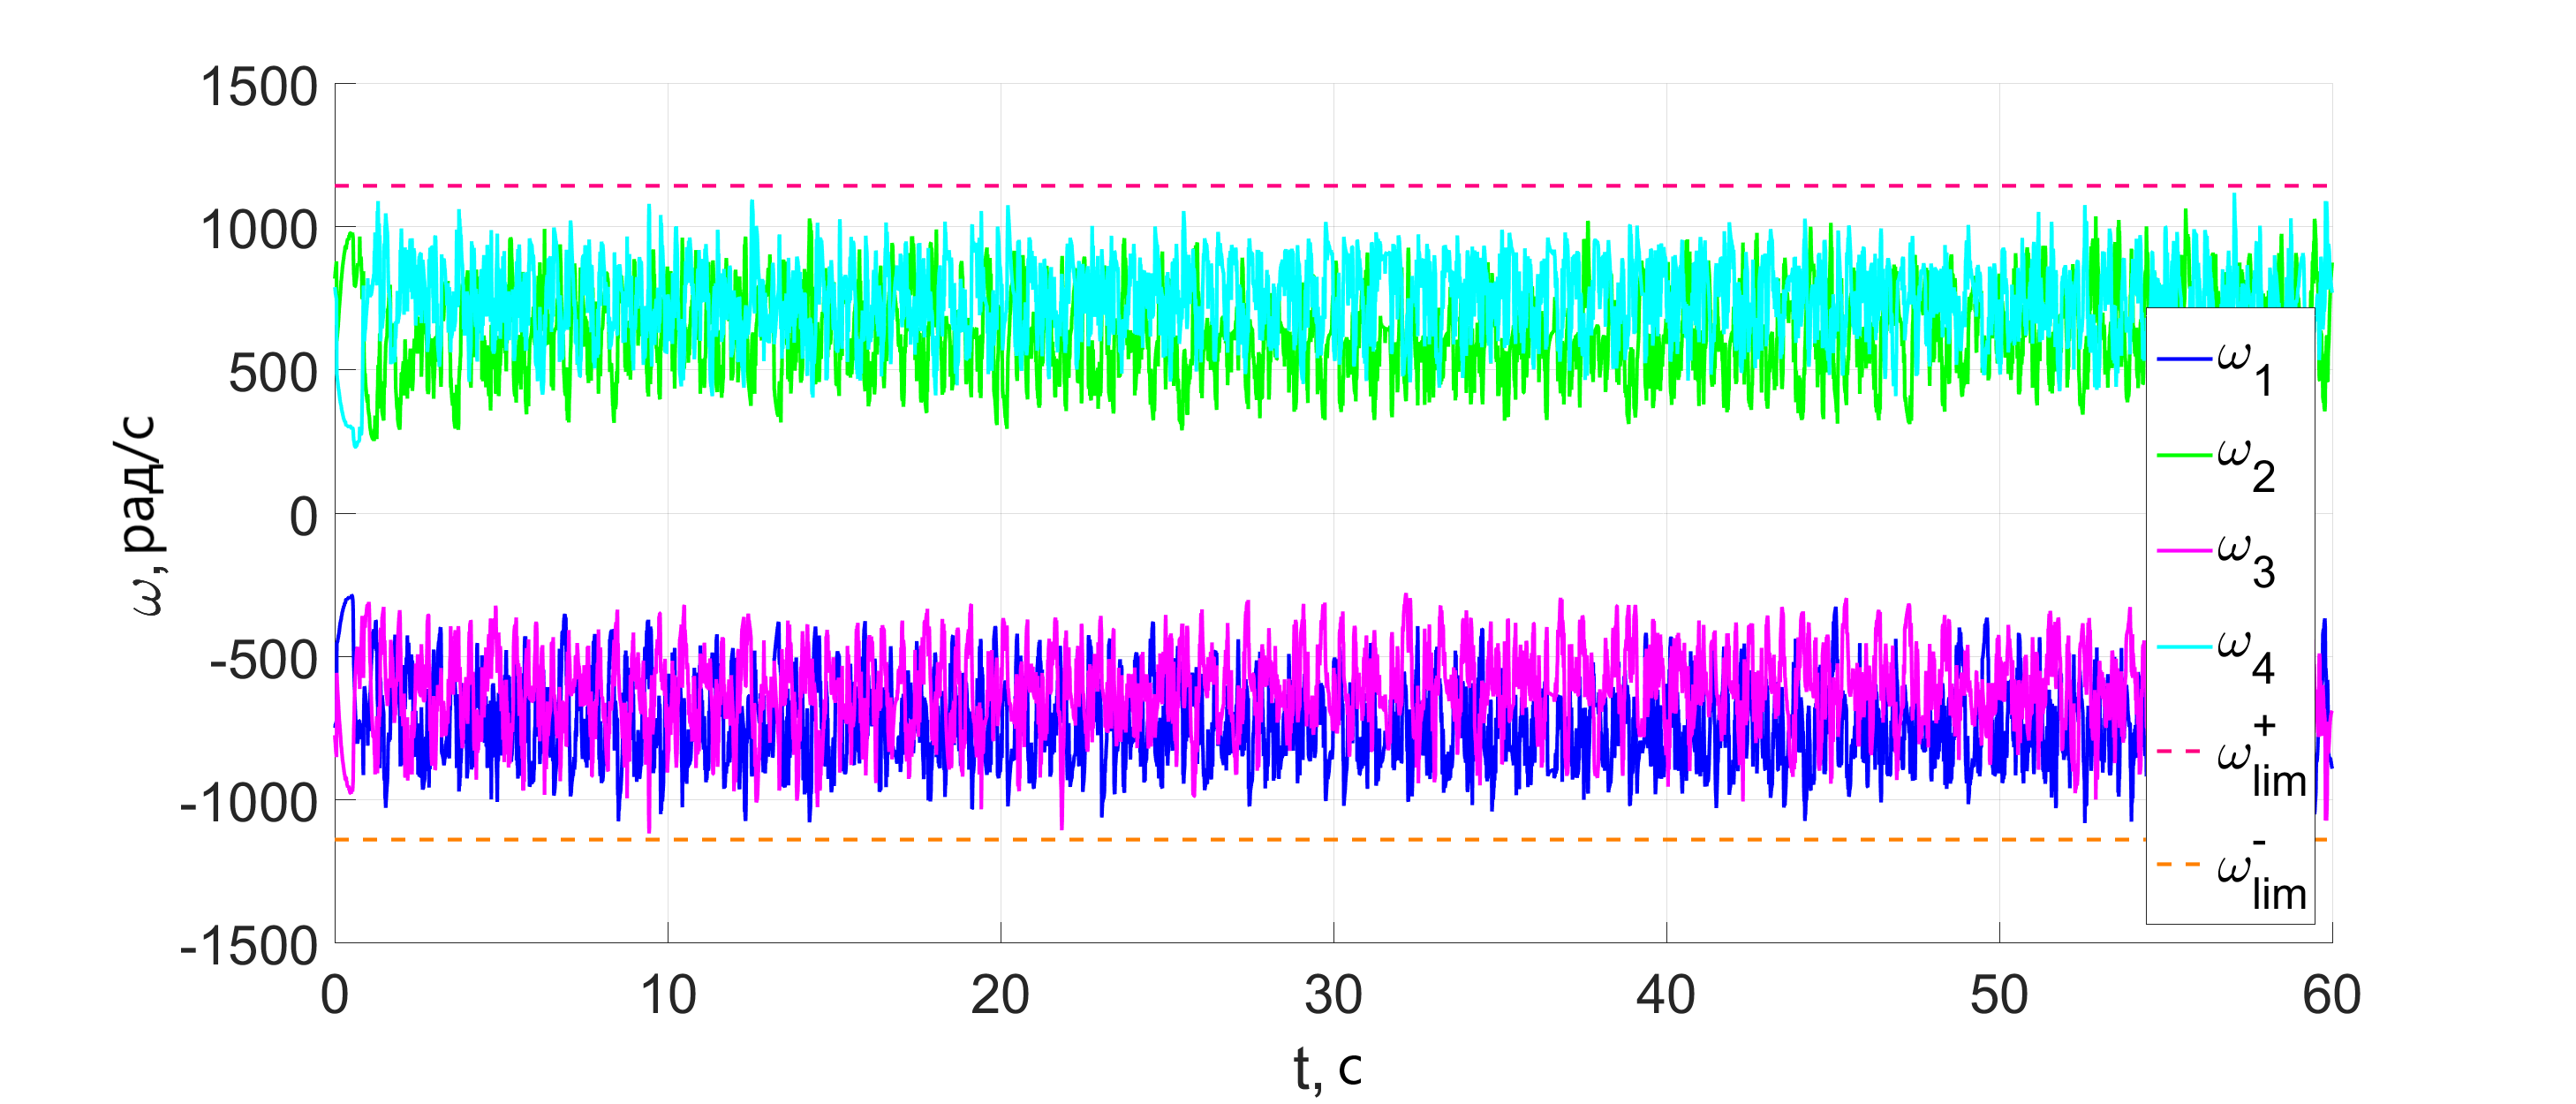
\includegraphics[clip,width=0.9\columnwidth]{omega}%
	}
	
	\subfloat[Углы отклонения сервоприводов]{%
		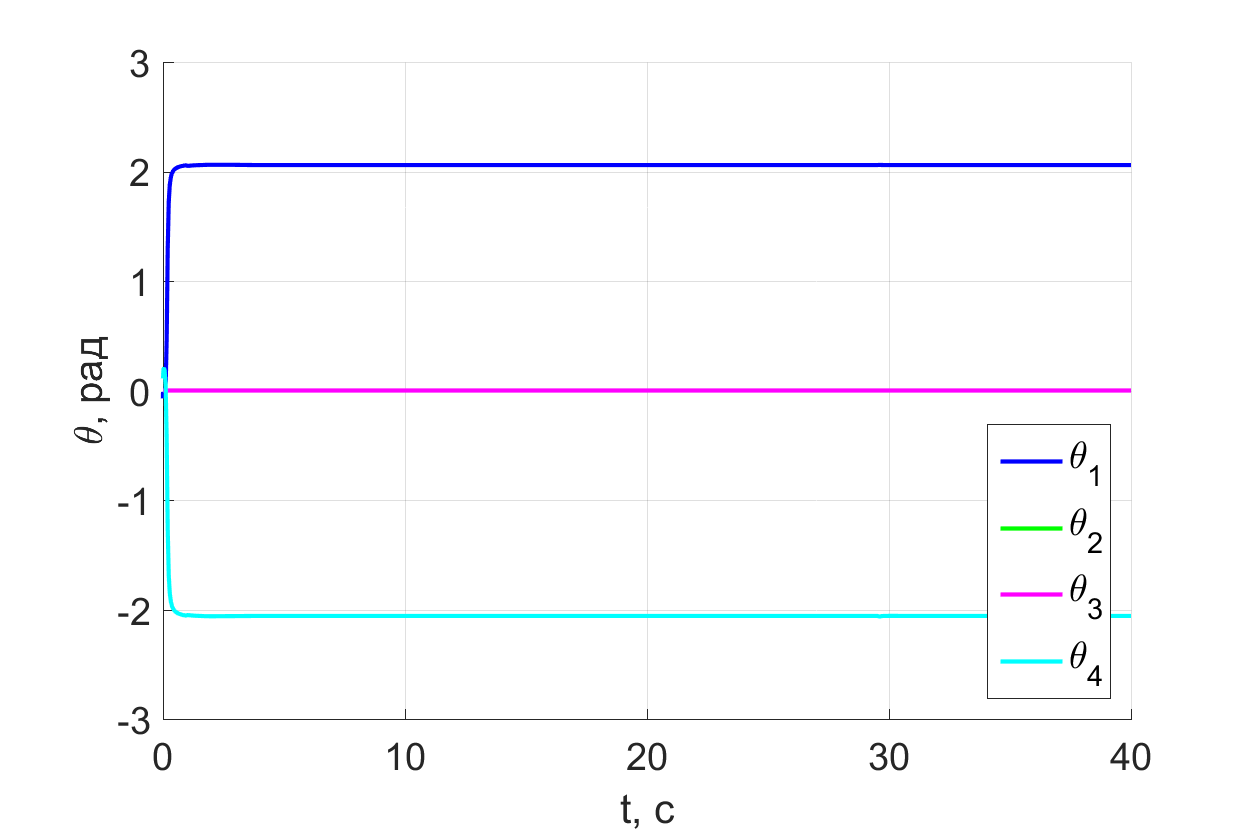
\includegraphics[clip,width=0.9\columnwidth]{theta}%
	}
	
	\caption{ -- Управляющие параметры}
	\label{fig:mau_ctrl_out}
	
\end{figure}

В результате эксперимента мы оценили способность БЛА с поворотными роторами справляться со сложными маневрами, где необходимо независимо управлять ориентацией и положением аппарата. Квадрокоптер быстро вышел на целевую траекторию и отслеживал ее с некоторой ошибкой, которая в основном обусловлена ошибкой оценки текущего положения.
Отметим, что для решения поставленной задачи наблюдения за подвижным объектом ошибка оказалась некритичной. 
Однако, при необходимости более точного отслеживания траектории имеет смысл использовать более чувствительные инструменты для измерения текущего положения и скорости, например, технологию RTK GPS \cite{Feng01}, где применение неподвижной наземной базовой станции уменьшает погрешность измерений на 1-2 порядка.